\documentclass[11pt, oneside]{article}   	% use "amsart" instead of "article" for AMSLaTeX format
\usepackage{geometry}                		% See geometry.pdf to learn the layout options. There are lots.
\geometry{letterpaper}                   		% ... or a4paper or a5paper or ... 
%\geometry{landscape}                		% Activate for for rotated page geometry
%\usepackage[parfill]{parskip}    		% Activate to begin paragraphs with an empty line rather than an indent
\usepackage{graphicx}				% Use pdf, png, jpg, or eps� with pdflatex; use eps in DVI mode
								% TeX will automatically convert eps --> pdf in pdflatex		
\usepackage{amssymb}
\usepackage{parskip}

\title{Trig substitutions}
%\author{The Author}
\date{}							% Activate to display a given date or no date
\graphicspath{{/Users/telliott_admin/Dropbox/Tex/png/}}

\begin{document}
\maketitle
%\section{}
%\subsection{}
\noindent
\Large

By now you've had plenty of experience with the trigonometric functions sine and cosine, and the others constructed from them like tangent and secant.  For example

\[ y = \sin \ \frac{\pi}{4} = \frac{1}{\sqrt{2}} \]

Here, we will consider the \emph{inverse} trigonometric functions.  That is, we use as our independent variable the value of the sine, and we ask which angle $\theta$ has that value for its sine (we can also use $y$ as the label for this variable, of course).  The function that yields the angle given the sine is called the inverse sine ($sin^{-1}$ or $arc sin$ or simply $asin$).

\[ y = \sin^{-1} (x) \]

or 

\[ \theta = \sin^{-1} (\frac{1}{\sqrt{2}}) \]
\[ \theta = \frac{\pi}{4} \]

Here is the figure from the wikipedia article on this topic showing the inverse sine and cosine.  (Recall that a function can assign only \emph{one} value of $y$ to each value of $x$.  Hence, the limits on the domain of the inverse sine function are $x = -1 \rightarrow 1$, and similarly for the inverse cosine.

\begin{center} \includegraphics [scale=0.5] {arcsin1.png} \end{center}

If we imagine the mirror image of the sine function rotated by 90 degrees (that is, both flipped and rotated), we obtain the inverse sine.  In the figure below, both hands are left hands, so in the left panel we are looking at the back of the hand, and in the right panel we are looking at the front or palm.

\begin{center} 
\includegraphics [scale=0.25] {hands.png} \end{center}

These two views have the same relationship as the sine and inverse sine (in fact, any function and its inverse have this property).


Below, both the sine and inverse sine are plotted.  They are symmetrical across the line $y=x$.

\begin{center} 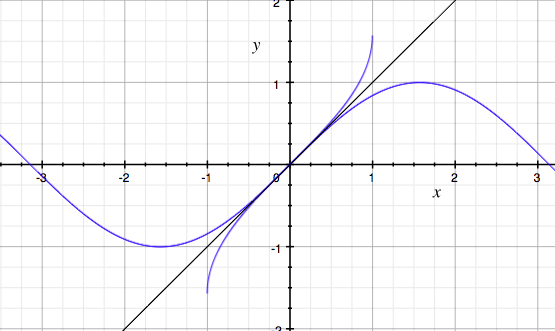
\includegraphics [scale=0.5] {arcsin2.png} \end{center}

The inverse trig functions might be no more than a curiosity, except that they provide solutions to some integrals.

Consider the figure below.  

\begin{center} 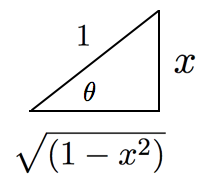
\includegraphics [scale=0.5] {trig1.png} \end{center}

\[
x = sin \ \theta
\]
\[
dx = cos\theta \ d\theta
\]
\[
\sqrt{1-x^2} = cos \ \theta
\]
So if we have an integral like
\[
\int \frac{x}{\sqrt{1-x^2} } \ dx
\]
substituting
\[
\int \frac{1}{cos\theta} \ sin\theta \ cos\theta \ d\theta = \int  sin\theta \ d\theta = -cos \theta = -\sqrt{1-x^2}
\]
Now, admittedly, we could also have done the integral by seeing that in the numerator we have the derivative of the $x^2$ squared term in the denominator, or by a more familiar type of substitution:
\[
u = 1-x^2
\]
\[
\ du = -2x \ dx
\]
\[
\int -\frac{1}{2} \  \frac{1}{\sqrt{u} } \ du = - \sqrt{u} = \ - \sqrt{1-x^2}
\]
But this is the basic idea of "trig substitutions".

The real advantage is that these substitutions allow us to integrate even when we don't have the derivative of what is under the square root sign.  Consider these two integrals
\[ \int \sqrt{1-x^2} \ dx, \ \ \ \ \  \int \frac{1}{\sqrt{1-x^2}} \ dx \]
with the substitution from before
\[  x = sin \ \theta\]
\[ dx = cos \ \theta \ d\theta\]
\[ \sqrt{1-x^2} = cos \ \theta \]
The second one is just
\[ \int \frac{1}{\sqrt{1-x^2}} \ dx = \int \frac{1}{cos \theta} \ cos \theta \ d \theta = \theta  = sin^{-1}x\]
while the first is the familiar
\[ \int \sqrt{1-x^2} \ dx = \int cos^2 \theta \ d \theta \]
\[ = \frac{1}{2} \ [ sin \theta \ cos \theta + \theta ] \]
\[ = \frac{1}{2} \ [x \ \sqrt{1-x^2}  + sin^{-1} x ]\]
which only becomes a little tricky in substituting back to x.

If we substitute a for 1 as the hypotenuse in the diagram, then we have
\[  x = a \ sin\theta \]
\[ dx = a \ cos\theta \ d\theta \] 
\[ \sqrt{(a^2-x^2)} = a \ cos\theta \]
and so
\[ \int \frac{1}{\sqrt{a^2-x^2}} \ dx \]
\[ = \int \frac{1}{a \ cos \theta} \ a \ cos \theta \ d \theta \]
\[ = \theta \ = sin^{-1} (\frac{x}{a}) \]
A definite integral requires consideration of the limits of integration.  For example, suppose the above example is
\[ x=0 \rightarrow x=a, \ \ \  a = 4 \]
What happens to $\theta$?
\[ \theta = \sin^{-1} \frac{x}{a} \]
when $x=0$, $\theta = 0$.  When $x = 4$, $x/a = 1$ and $\theta = \pi/2$.

All the integrals above involve $\sqrt{a^2-x^2}$ or $\sqrt{1-x^2}$.  For any of these, if we can work an example with $a=1$, we can work it for any constant $a$.

\subsection*{Other types}

Two other classes are those with $\sqrt{x^2 + a^2}$ and $\sqrt{x^2-a^2}$.  

For the first type we should put $x$ as the side opposite $\theta$, $a$ as the side adjacent, and $\sqrt{x^2 + a^2}$ as the hypotenuse.

\[ x = a\ \tan \ \theta \]
\[ dx = a \ \sec^2 \theta \ d \theta \]
\[ \theta = \tan^{-1} (\frac{x}{a}) \]
\[ \int \frac{1}{x^2 + a^2} \ dx = \int \frac{1}{a^2 \ \tan^2 \theta + a^2} \ a \ \sec^2 \theta \ d \theta \]
Notice that $\sec^2 = 1 + \tan^2 \theta$ so
\[ = \frac{1}{a} \ \int d \theta = \frac{1}{a} \ \theta = \frac{1}{a} \tan^{-1}(\frac{x}{a}) \]

\subsection*{The last type}

\[ \int \sqrt{x^2-a^2} \ dx \]

In this case, we will have $x$ as the hypotenuse, $a$ as the side adjacent to $\theta$, and $\sqrt{x^2 - a^2}$ as the side opposite.

We have 
\[ \frac{1}{a} \sqrt{x^2-a^2} = \tan \theta \]
\[ \sqrt{x^2-a^2} = a \tan \theta \]
\[ \frac{1}{a} x = \sec \theta \]
\[  dx = a \sec \theta \tan \theta \ d \theta \]

So we have
\[ \int \sqrt{x^2-a^2} \ dx \]
\[ = a^2 \int \sec \theta \tan^2 \theta \ d \theta \]

using the familiar identity $1 + \tan^2 \theta = \sec^2 \theta $:
\[ = a^2 \int \sec \theta \ (\sec^2 \theta - 1) \ d \theta \]
\[ = a^2 \int (\sec^3 \theta - \sec \theta) \  d\theta \]
which is a bit tricky.  If you look it up in a table of integrals, the individual answers are
\[ \int \sec \ x \ dx = \ln | \sec x + \tan x| \]
\[ \int \sec^3 x \ dx = \frac{1}{2}(\sec x \ \tan x + \ln | \sec x + \tan x|) \]

\subsection*{Actually doing the integrals}
When faced with 
\[ \int \sec x \ dx \]
somebody once had a wild idea!  Multiply and divide by $\tan x + \sec x$:
\[ \int \sec x \ \frac{\tan x + \sec x}{\tan x + \sec x}  \ dx \]
\[ =  \int \frac{\sec x \ \tan x + \sec^2 x}{\sec x + \tan x}  \ dx \]
Recall that the derivative of $\tan x$ is $\sec^2 x$ and the derivative of $\sec x$ is $\sec x \tan x$.

Our clever construction has produced an expression

\[ =  \int \frac{\sec x \ \tan x + \sec^2 x}{\sec x + \tan x}  \ dx \]

 in which the numerator is the derivative of the denominator.  This is just
\[ \int \frac{1}{u} \ du = \ln |u| \]
\[ = \ln |\sec x + \tan x| \]
plus $C$, of course.

We can certainly check that.
\[ \frac{d}{dx} \ln |\sec x + \tan x| \]
\[ = \frac{1}{\sec x + \tan x} \ (\sec x \tan x + \sec^2 x) \]
\[ = \sec x \ \frac{\tan x + \sec x}{\sec x + \tan x}  \]
\[ = \sec x \]

\subsection*{Actually doing the cubed secant}
We start by recalling that $\sec^2 x = 1 + \tan^2 x$, so

\[ \int  \sec^3 x \ dx \]
\[ = \int \sec x \ (1 + \tan^2 x) \ dx \]
\[ = \int \sec x \ dx + \int \sec x \tan^2 x \ dx \]

To do the right-hand expression, we use integration by parts
\[ u = \tan x \]
\[ du = \sec^2 x \ dx \]
\[ dv = \sec x \tan x \ dx \]
\[ v = \sec x \]
So what we have above (in the second term on the right) is $\int u \ dv$ and we get:
\[ = uv - \int v \ du \]
\[ = \sec x \tan x - \int \sec^3 x \ dx \]
Seems like we are back where we started, except .. 

Let's write out the whole thing:
\[ \int  \sec^3 x \ dx = \int \sec x \ dx + \int \sec x \tan^2 x \ dx \]
\[ \int  \sec^3 x \ dx = \ln |\sec x + \tan x| + \sec x \tan x - \int \sec^3 x \ dx \]
So
\[ 2 \int  \sec^3 x \ dx = \ln |\sec x + \tan x| + \sec x \tan x  \]
\[ \int  \sec^3 x \ dx = \frac{1}{2} \ [ \ \ln |\sec x + \tan x| + \sec x \tan x  \ ]  \]
We developed a similar argument with $\int \cos^2 x \ dx$, if you remember.

To check it (save the $1/2$ for later):
\[ \frac{d}{dx} \ \ln |\sec x + \tan x| + \sec x \tan x  \]
\[ = \frac{1}{\sec x + \tan x} (\sec x \ \tan x + \sec^2 x) + \sec^3 x + \sec x \tan^2 x \]
\[ = \sec x + \sec^3 x + \sec x \tan^2 x \]
\[ = \sec x + \sec^3 x + \sec x (\sec^2 x - 1) \]
\[ = 2 \sec^3 x  \]
The extra factor of $1/2$ makes it exactly correct.



\end{document}  